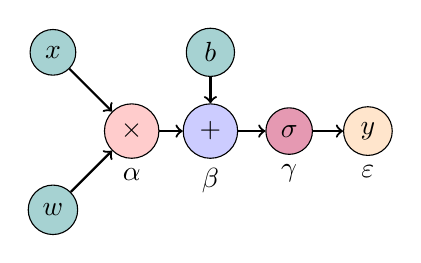
\begin{tikzpicture}[node distance=1cm]
    \node[draw, circle, fill=red!20, label=below:$\alpha$] (multiply) {$\times$};
    \node[draw, circle, fill=blue!20, right of=multiply, label=below:$\beta$] (addition) {$+$};
    \node[draw, circle, fill=purple!40, right of=addition, label=below:$\gamma$] (function) {$\sigma$};
    \node[draw, circle, fill=orange!20, right of=function, label=below:$\varepsilon$] (output) {$y$};

    \draw[->, thick] (multiply) -- (addition);
    \draw[->, thick] (addition) -- (function);
    \draw[->, thick] (function) -- (output);

    \node[draw, circle, fill=teal!35, left of=multiply, yshift=1cm] (input1) {$x$};
    \node[draw, circle, fill=teal!35, left of=multiply, yshift=-1cm] (input2) {$w$};
    \node[draw, circle, fill=teal!35, left of=addition, yshift=1cm, xshift=1cm] (bias) {$b$};

    \draw[->, thick] (input1) -- (multiply);
    \draw[->, thick] (input2) -- (multiply);
    \draw[->, thick] (bias) -- (addition);
\end{tikzpicture}